\section{Voice Cloning}
Kloning suara sering diombang-ambingkan dengan istilah lain, seperti suara deepfake, sintesis ucapan, dan suara sintetis, yang memiliki arti yang sedikit berbeda. Kloning suara adalah proses di mana seseorang menggunakan komputer untuk menghasilkan ucapan individu nyata, menciptakan tiruan dari suara mereka yang spesifik dan unik menggunakan kecerdasan buatan (AI)\cite{8999436}. Sistem text-to-speech (TTS), yang dapat mengambil bahasa tertulis dan mengubahnya menjadi komunikasi lisan, tidak sama dengan kloning suara. Sistem TTS jauh lebih terbatas dari output yang mereka hasilkan dibandingkan dengan teknologi kloning suara, yang sebenarnya lebih merupakan proses kustom. Dengan sistem TTS, data pelatihan, komponen kunci untuk setiap media yang dibuat secara sintetis, menginformasikan produksi keluaran suara. Dengan kata lain, suara yang Anda dengar adalah suara yang diberikan dalam kumpulan data. Sekarang, dengan diperkenalkannya teknologi AI kloning suara, itu berubah. Metode telah diterapkan untuk memberikan analisis yang lebih dalam dan ekstraksi karakteristik suara target. Atribut-atribut ini kemudian dapat diterapkan pada bentuk gelombang ucapan yang berbeda, memungkinkan seseorang untuk mengubah keluaran suara dari satu suara ke suara lainnya\cite{9239750}.

\begin{figure}[H]
        \centerline{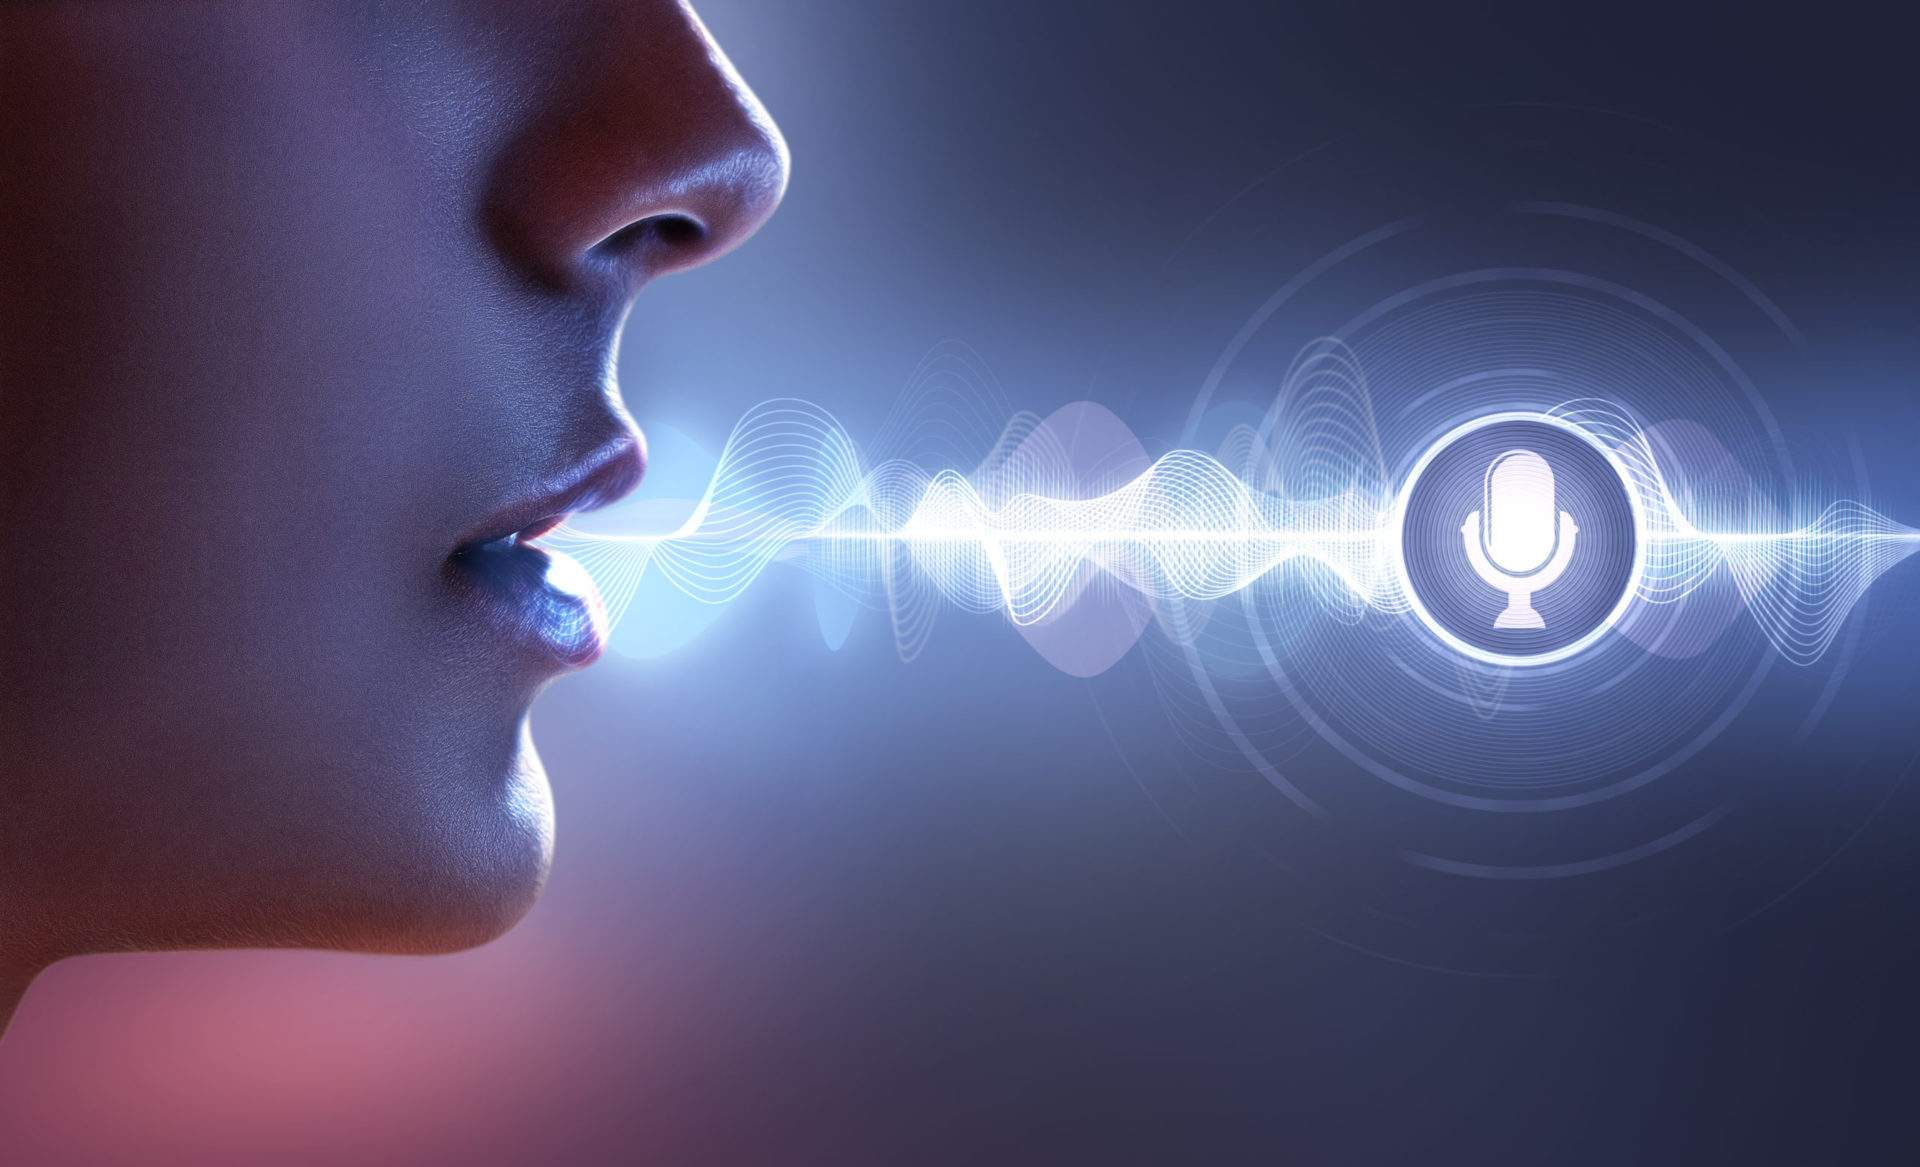
\includegraphics[scale=.15]{figures/voicecloning}}
        \caption{Voice Cloning}
		\label{voicecloning}
\end{figure}

Berkat kemajuan dalam kecerdasan buatan (AI), khususnya pembelajaran mendalam, bagian dari pembelajaran mesin di bawah payung AI, kami telah mampu menghasilkan replika suara yang akurat. Tapi ini hanya dimungkinkan oleh dua hal:

\begin{enumerate}
\item Perangkat keras yang kuat dengan kemampuan komputasi awan untuk memproses dan merender secara tepat waktu dan efisien
\item Data pelatihan ekstensif dari suara yang ditargetkan dari mana model dapat memanfaatkan untuk membuat klon suara yang akurat
\end{enumerate}

Dengan AI yang tepat dan keahlian dan alat pengembangan, itu benar-benar tergantung pada yang terakhir. Anda memerlukan sejumlah besar ucapan yang direkam untuk memiliki data yang cukup untuk melatih model suara. Informasi seputar suara disimpan dalam embedding , ruang berdimensi cukup rendah di mana Anda dapat menerjemahkan variabel diskrit menjadi vektor berdimensi tinggi. Dengan kata lain, lebih mudah untuk bekerja dengan input besar dengan model pembelajaran mesin. Agar tidak terlalu teknis, kami akan berhenti di situ, tetapi jangan ragu untuk menyelam lebih dalam ke subjek jika itu menarik minat Anda.

\subsection{Manfaat Voice Cloning}
Mari kita mulai dengan yang baik. Ada banyak kasus penggunaan potensial untuk kloning suara yang sering kali dibayangi oleh penggunaan negatif, yang akan kita bahas sebentar lagi. Beberapa aplikasi positif dari teknologi meliputi:

\begin{enumerate}
\item Meningkatkan peluang iklan dan sponsor untuk pengisi suara, selebritas, dan influencer
\item Bantu perusahaan bekerja dengan talenta selama waktu tersibuk mereka dalam setahun, seperti musim sepak bola untuk pemain atau pelatih
\item Menghidupkan kembali suara-suara dari masa lalu untuk digunakan dalam hiburan guna membantu menceritakan kisah dalam dokumenter, film, dan acara TV
\item Diversifikasi konten siaran untuk konten berulang seperti laporan cuaca atau pembaruan olahraga
\item Lokalkan konten sehingga dapat didengar dalam suara pembawa acara atau narator dalam bahasa lain
\end{enumerate}

Ini hanyalah beberapa kegunaan positif dari kloning suara, dan seiring dengan berkembangnya teknologi, lebih banyak lagi yang akan muncul. Tapi tentu saja, semuanya bergantung pada etika penggunaan suara seseorang. Itulah mengapa perlunya gerakan menuju standarisasi proses persetujuan sangat penting untuk melindungi suara semua orang dan memastikan mereka memiliki kendali penuh atas cara penggunaannya.

\subsection{Aplikasi Voice Cloning Terbaik}

\begin{figure}[H]
        \centerline{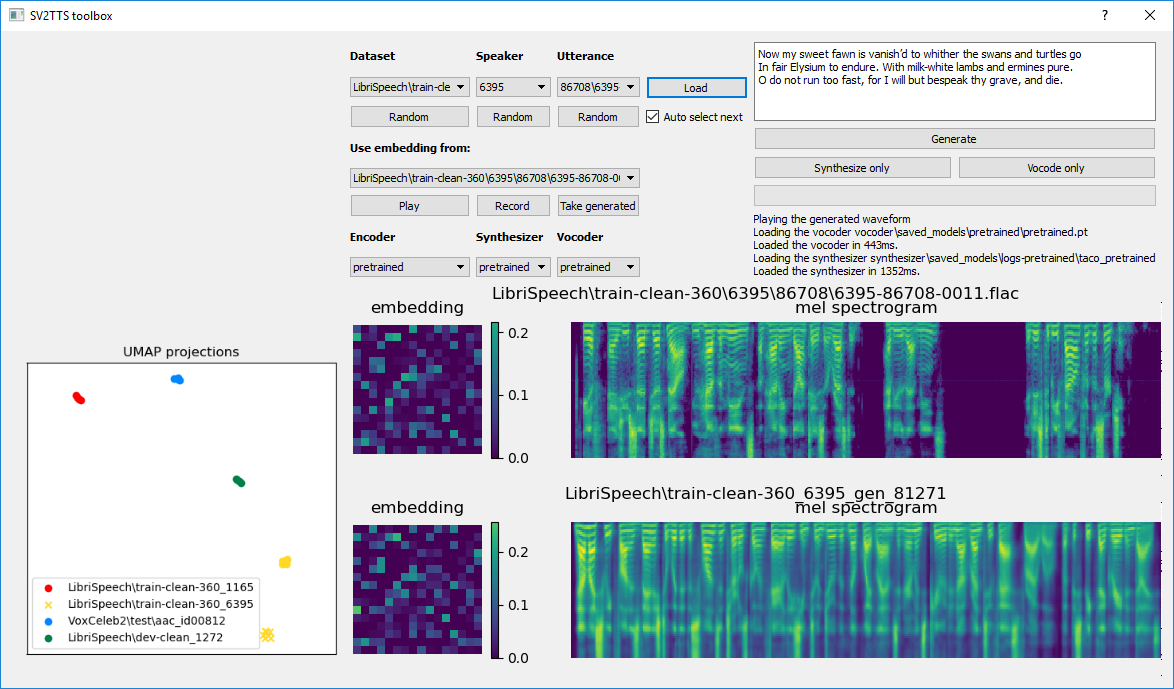
\includegraphics[scale=.35]{figures/voice-clone}}
        \caption{Contoh Aplikasi Voice Cloning (SV2TTS Toolbox)}
		\label{appvoice}
\end{figure}

Untuk mempersempit pencarian Anda untuk menemukan aplikasi kloning suara terbaik, Anda harus terlebih dahulu menentukan apa yang Anda cari. Apakah Anda memerlukan sesuatu yang lebih untuk output text-to-speech? Atau apakah Anda membutuhkan sesuatu yang lebih khusus?

Setelah Anda mengetahui mengapa Anda memerlukan aplikasi kloning suara, Anda harus mengasah tiga kriteria utama:
\begin{enumerate}
\item Kualitas keluaran: Anda pasti ingin memastikan bahwa keluaran terdengar otentik dan memenuhi kebutuhan yang ditentukan. Biasanya, mereka akan memiliki sampel tentang apa yang dapat dilakukan produk tersebut. Jika tidak, Anda harus mempertimbangkan untuk meminta demo, jika tersedia, untuk menentukan seberapa manusiawi produk mereka.

\item Antarmuka intuitif: seberapa mudah menggunakan aplikasi? Apakah sulit untuk menemukan sesuatu saat Anda berada di aplikasi atau dapatkah Anda menavigasi dan menggunakannya untuk memenuhi kebutuhan Anda? Sekali lagi, ini dapat ditentukan oleh video produk, konten pemasaran, dan demo.

\item Perlindungan suara: Anda pasti ingin memastikan bahwa perusahaan mengikuti penggunaan suara yang etis. Jika itu adalah layanan kustom yang memerlukan data pelatihan, maka penting untuk menanyakan tentang perlindungan data dan bagaimana suara, saat dibuat, tidak akan digunakan secara tidak semestinya.
\end{enumerate}

Implikasi etis seputar kloning suara adalah hubungan dari Veritone MARVEL.ai, aplikasi suara sebagai layanan kami . Dibangun dalam kerangka aplikasi adalah tuas untuk memberi pengguna kendali atas suara mereka, memungkinkan perlindungan yang tepat sehingga mereka memutuskan siapa yang dapat menggunakan suara mereka. Ini membantu kami memberikan solusi voice-as-a-service khusus kami untuk memungkinkan pengalaman sarung tangan putih lengkap untuk talenta yang bekerja dengan kami.

\subsection{Pembuatan Voice Cloning}
Perangkat lunak kloning suara AI online dimulai dengan menggunakan komputer untuk mensintesis suara. Text-to-Speech (TTS) adalah teknologi berusia puluhan tahun yang mengubah teks menjadi ucapan sintetis, memungkinkan suara digunakan untuk interaksi komputer-manusia.

Di masa lalu ada dua pendekatan untuk TTS. Yang pertama, TTS Concatenative\cite{Hunt1996UnitSI}, menggunakan rekaman audio untuk membuat perpustakaan kata dan satuan suara (fonem) yang dapat dirangkai menjadi kalimat. Meskipun keluarannya berkualitas tinggi dan dapat dipahami, ia tidak memiliki emosi dan infleksi yang ditemukan dalam ucapan manusia yang alami. Saat menggunakan TTS Concatenative, setiap gaya bicara atau bahasa baru memerlukan database audio baru. Dan tentu saja upaya untuk mengkloning suara individu menggunakan metode ini membutuhkan investasi yang sangat besar, biasanya hanya dilakukan untuk mendukung suara bermerek.

Pendekatan kedua adalah Parametrik TTS\cite{ZEN20091039}, metode yang menggunakan model statistik ucapan untuk menyederhanakan pembuatan suara, mengurangi biaya dan upaya dibandingkan dengan Penggabungan. Namun, upaya untuk menciptakan satu suara apa pun secara historis mahal, dan hasilnya jelas bukan manusia.

Saat ini, Kecerdasan Buatan (AI) dan kemajuan dalam Pembelajaran Mendalam meningkatkan kualitas ucapan sintetis. Pengajuan TTS sekarang sudah lumrah. Setiap orang yang telah berinteraksi dengan sistem Respon Suara Interaktif berbasis telepon, Siri Apple, Amazon Alexa, sistem navigasi mobil, atau banyak antarmuka suara lainnya, telah mengalami ucapan sintetis.

Jika Anda terbiasa dengan konsep video deepfake, perangkat lunak kloning suara AI online adalah setara dengan ucapan. Hanya dengan beberapa menit rekaman ucapan, pengembang dapat membangun kumpulan data audio dan menggunakannya untuk melatih model suara AI yang dapat membaca teks apa pun dalam suara target.

Pembuatan voice cloning secara signifikan menjadi lebih mudah berkat berbagai alat bertenaga jaringan saraf seperti Tacotron dan Wavenet atau Lyrebird Google, yang memungkinkan hampir semua suara direplikasi dan digunakan untuk "membaca" input teks. Kualitas output terus meningkat, seperti yang ditunjukkan oleh tiruan suara podcaster Joe Rogan ini. Insinyur pembelajaran mendalam di Dessa yang membuat klon juga menyiapkan kuis. Ambil untuk melihat apakah Anda dapat melihat Rogan palsu.

Model TTS berbasis jaringan saraf meniru cara otak beroperasi dan sangat efisien dalam mempelajari pola dalam data. Meskipun ada pendekatan berbeda untuk penggunaan pembelajaran mendalam dalam suara sintetis, sebagian besar menghasilkan pengucapan kata yang lebih baik, serta menangkap kehalusan seperti kecepatan dan intonasi untuk menciptakan ucapan yang lebih mirip manusia. 

Penting untuk dicatat bahwa alat yang disebutkan di atas dan alat lain seperti ini tidak dibuat untuk tujuan penipuan atau penipuan. Tetapi kenyataannya adalah bahwa bisnis dan konsumen perlu mewaspadai ancaman baru yang terkait dengan perangkat lunak kloning suara AI online. Kami menjelajahi beberapa kegunaan — baik dan buruk — di bawah ini. 

\subsection{Dampak Negatif Voice Cloning}
\begin{enumerate}
\item Voice adalah pengenal pribadi unik yang mudah diakses oleh penipu. Hal ini tentu berlaku bagi publik figur termasuk selebriti, politisi dan pemimpin bisnis, tetapi kenyataannya adalah siapa saja bisa menjadi sasaran. Video online, pidato, panggilan konferensi, percakapan telepon, dan posting media sosial semuanya dapat digunakan untuk mengumpulkan data yang diperlukan untuk melatih sistem untuk mengkloning suara.

\item Spoofing biometrik suara — Suara adalah pengidentifikasi unik dan ukuran yang andal untuk keamanan biometrik. Namun, penjahat dapat menggunakan serangan presentasi termasuk suara yang direkam, suara yang diubah komputer dan suara sintetis, atau kloning suara, untuk mengelabui sistem biometrik suara agar mengira mereka mendengar pengguna yang sebenarnya dan berwenang dan memberikan akses ke informasi dan akun sensitif.
\begin{figure}[H]
        \centerline{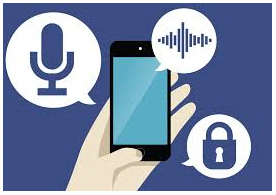
\includegraphics[scale=1]{figures/spoof}}
        \caption{Spoofing Voice Biometrics}
		\label{spoof}
\end{figure}

\item Penipuan phishing – Perangkat lunak kloning suara AI online juga memungkinkan jenis baru penipuan phishing yang mengeksploitasi fakta bahwa korban percaya bahwa mereka sedang berbicara dengan seseorang yang mereka percayai. Tahun lalu, seorang CEO yang berbasis di Inggris ditipu untuk mentransfer lebih dari \$240.000 berdasarkan panggilan telepon yang dia yakini berasal dari bosnya, CEO perusahaan induk organisasi Jerman.
\begin{figure}[H]
        \centerline{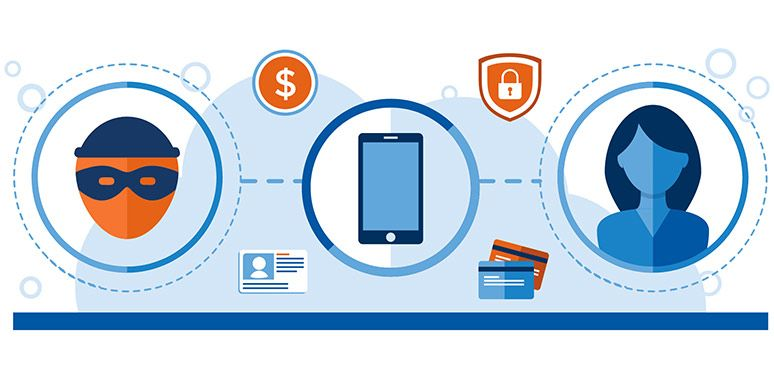
\includegraphics[scale=.4]{figures/voice-phising}}
        \caption{Voice Phising, Sumber: \url{https://id.pinterest.com/pin/195765915039905230/}}
		\label{phising}
\end{figure}

\item Penipuan seperti ini adalah evolusi penipuan email di mana email eksekutif dipalsukan dalam upaya agar penerima membocorkan nomor rekening bank, informasi kartu kredit, kata sandi, dan data sensitif lainnya. Sekarang scammers, dipersenjatai dengan klon suara, menggunakan panggilan telepon dan pesan suara. Dan serangan itu tidak hanya mengancam bisnis. Dalam generasi baru penjahat "mother's deception" menyamar sebagai anggota keluarga yang membutuhkan dana darurat.

\item Misinformasi – Berita palsu dan bentuk misinformasi serupa merupakan ancaman serius. Banyak dari kita yang akrab dengan bagaimana video yang dimanipulasi berdampak pada lanskap politik. Misalnya, video populer menunjukkan Barack Obama memanggil Trump – yah, anggap saja itu tidak terlalu bagus. Itu juga tidak nyata. Teknologi perangkat lunak text-to-speech berbasis AI akan semakin mendorong upaya ini untuk mempengaruhi opini publik, menghidupkan sumbangan kampanye palsu, mencemarkan nama baik tokoh masyarakat, dan banyak lagi. Di bidang bisnis, pertimbangkan bagaimana pernyataan eksekutif atau figur publik yang dimanipulasi dapat memengaruhi pasar saham.

\item Bukti – Suara sintetis dan deepfake lainnya dapat digunakan untuk membuat bukti palsu yang berdampak pada kasus kriminal. Meskipun ada pemeriksaan untuk memvalidasi bukti audio dan video yang disajikan di pengadilan, mencegah taktik ini memengaruhi kesaksian berdasarkan apa yang orang yakini mereka lihat atau dengar mungkin merupakan tantangan.

\item Pemerasan dan intimidasi – Video dan audio yang dimanipulasi dari orang-orang yang melakukan atau mengatakan hal-hal yang tidak mereka katakan dapat digunakan untuk intimidasi online dan ancaman untuk mengekspos konten palsu dan memalukan jika korban menolak untuk membayar biaya.

\end{enumerate}

\subsection{Dampak Positif Voice Cloning}
\begin{enumerate}
\item Pendidikan, Mengkloning suara tokoh sejarah menawarkan peluang baru untuk pengajaran interaktif dan penceritaan yang dinamis. Misalnya, pada 22 November 1963 Presiden Kennedy sedang dalam perjalanan untuk memberikan pidato di Dallas ketika dia dibunuh. Kita sekarang dapat mendengar pidato itu dengan kata-katanya sendiri menggunakan teknologi deepfake. Dalam penggunaan deepfake AI lainnya yang menakjubkan, pengunjung Museum Dalí di St. Petersburg akan disambut oleh Salvador Dali sendiri. Dali berinteraksi dengan tamu menggunakan kutipan aktual dan membuat komentar, dan bahkan berfoto selfie dengan mereka. Lihat video dan pelajari lebih lanjut tentang bagaimana Dali dihidupkan kembali melalui kekuatan AI. 

\item Audiobooks, Menggunakan perangkat lunak kloning suara AI, suara selebriti dapat digunakan untuk menceritakan buku, otobiografi dapat dibaca oleh penulis, dan tokoh sejarah dapat menceritakan kisah mereka dengan suara mereka sendiri. Hasilnya adalah pengalaman mendengarkan yang imersif dan berkualitas tinggi.

\item Assistive Tech, Suara sintetis dapat digunakan untuk membantu penyandang disabilitas atau masalah kesehatan yang memengaruhi kemampuan bicara mereka. Misalnya, orang yang tunarungu atau menderita gangguan seperti Penyakit Parkinson atau ALS dapat meningkatkan kemampuan mereka untuk berkomunikasi menggunakan versi sintetis dari suara dan TTS mereka.

\item Voice Branding, menggunakan suara pribadi dan khusus  sebagai merek utama perusahaan Anda dalam asisten percakapan dan aktivitas pemasaran Anda.

\item Digital Dubbing and Animation, Kloning suara memungkinkan untuk membuat suara yang dapat diidentifikasi untuk karakter digital unik atau avatar dalam sistem interaksi manusia-komputer atau untuk produksi konten multimedia dan audiovisual.

\item Smart Assistant, Suara smart assistant terdengar semakin alami karena kemajuan di bidang AI teknologi text-to-speech. Kloning suara memungkinkan personalisasi mereka, melalui penggunaan suara tertentu atau favorit untuk mengembangkan asisten percakapan yang disesuaikan.
\begin{figure}[H]
        \centerline{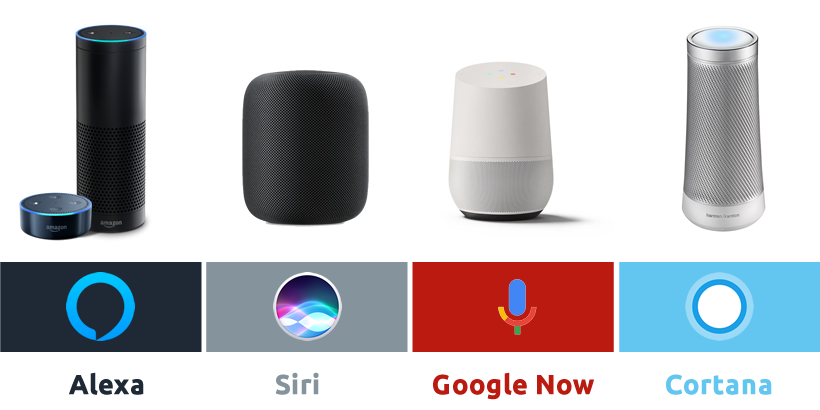
\includegraphics[scale=.45]{figures/voice-assistants-battle}}
        \caption{Smart Assistant, Sumber: https://blog.evolvemachinelearners.com/voice-assistant-its-history-twist-and-turn/}
		\label{assistant}
\end{figure}

\end{enumerate}

\subsection{Mendeteksi Deepfake Voice}
Karena teknologi suara terus meningkat, memiliki teknologi yang dapat mengenali dan menghentikan penggunaan ucapan palsu untuk penipuan dan penipuan sangat penting. 

Anti-spoofing suara, juga disebut deteksi keaktifan suara, adalah teknologi yang mampu membedakan antara suara langsung dan suara yang direkam, dimanipulasi, atau sintetis. Banyak pemalsuan saat ini tidak terlihat oleh telinga manusia, tetapi dapat dideteksi oleh perangkat lunak berbasis AI yang dilatih untuk mengidentifikasi artefak yang tidak ada dalam suara langsung. 

Teknologi yang mendeteksi perangkat lunak kloning suara AI pada awalnya dibuat untuk memecahkan masalah spoofing biometrik suara. Di mana biometrik suara mencocokkan suara seseorang dengan templat suara pada file, teknologi anti-spoofing memeriksa untuk memastikan suara itu hidup. Teknologi ini akan terus beradaptasi untuk mengatasi kasus penggunaan tambahan karena penipuan kloning suara menjadi lebih umum. Topik tersebut bahkan menjadi fokus lokakarya FTC baru -baru ini dengan peserta dari ID R\&D DARPA, University of Florida, MIT Sloan School of Management, dan program Defending Democracy dari Microsoft.

